\subsubsection{Benutzeransicht}
\label{sec:Benutzeransicht}

Ein erster Oberflächenentwurf der Benutzeransicht des vorliegenden Projektes ist in folgender Abbildung zu sehen.

\begin{figure}[htb]
\centering
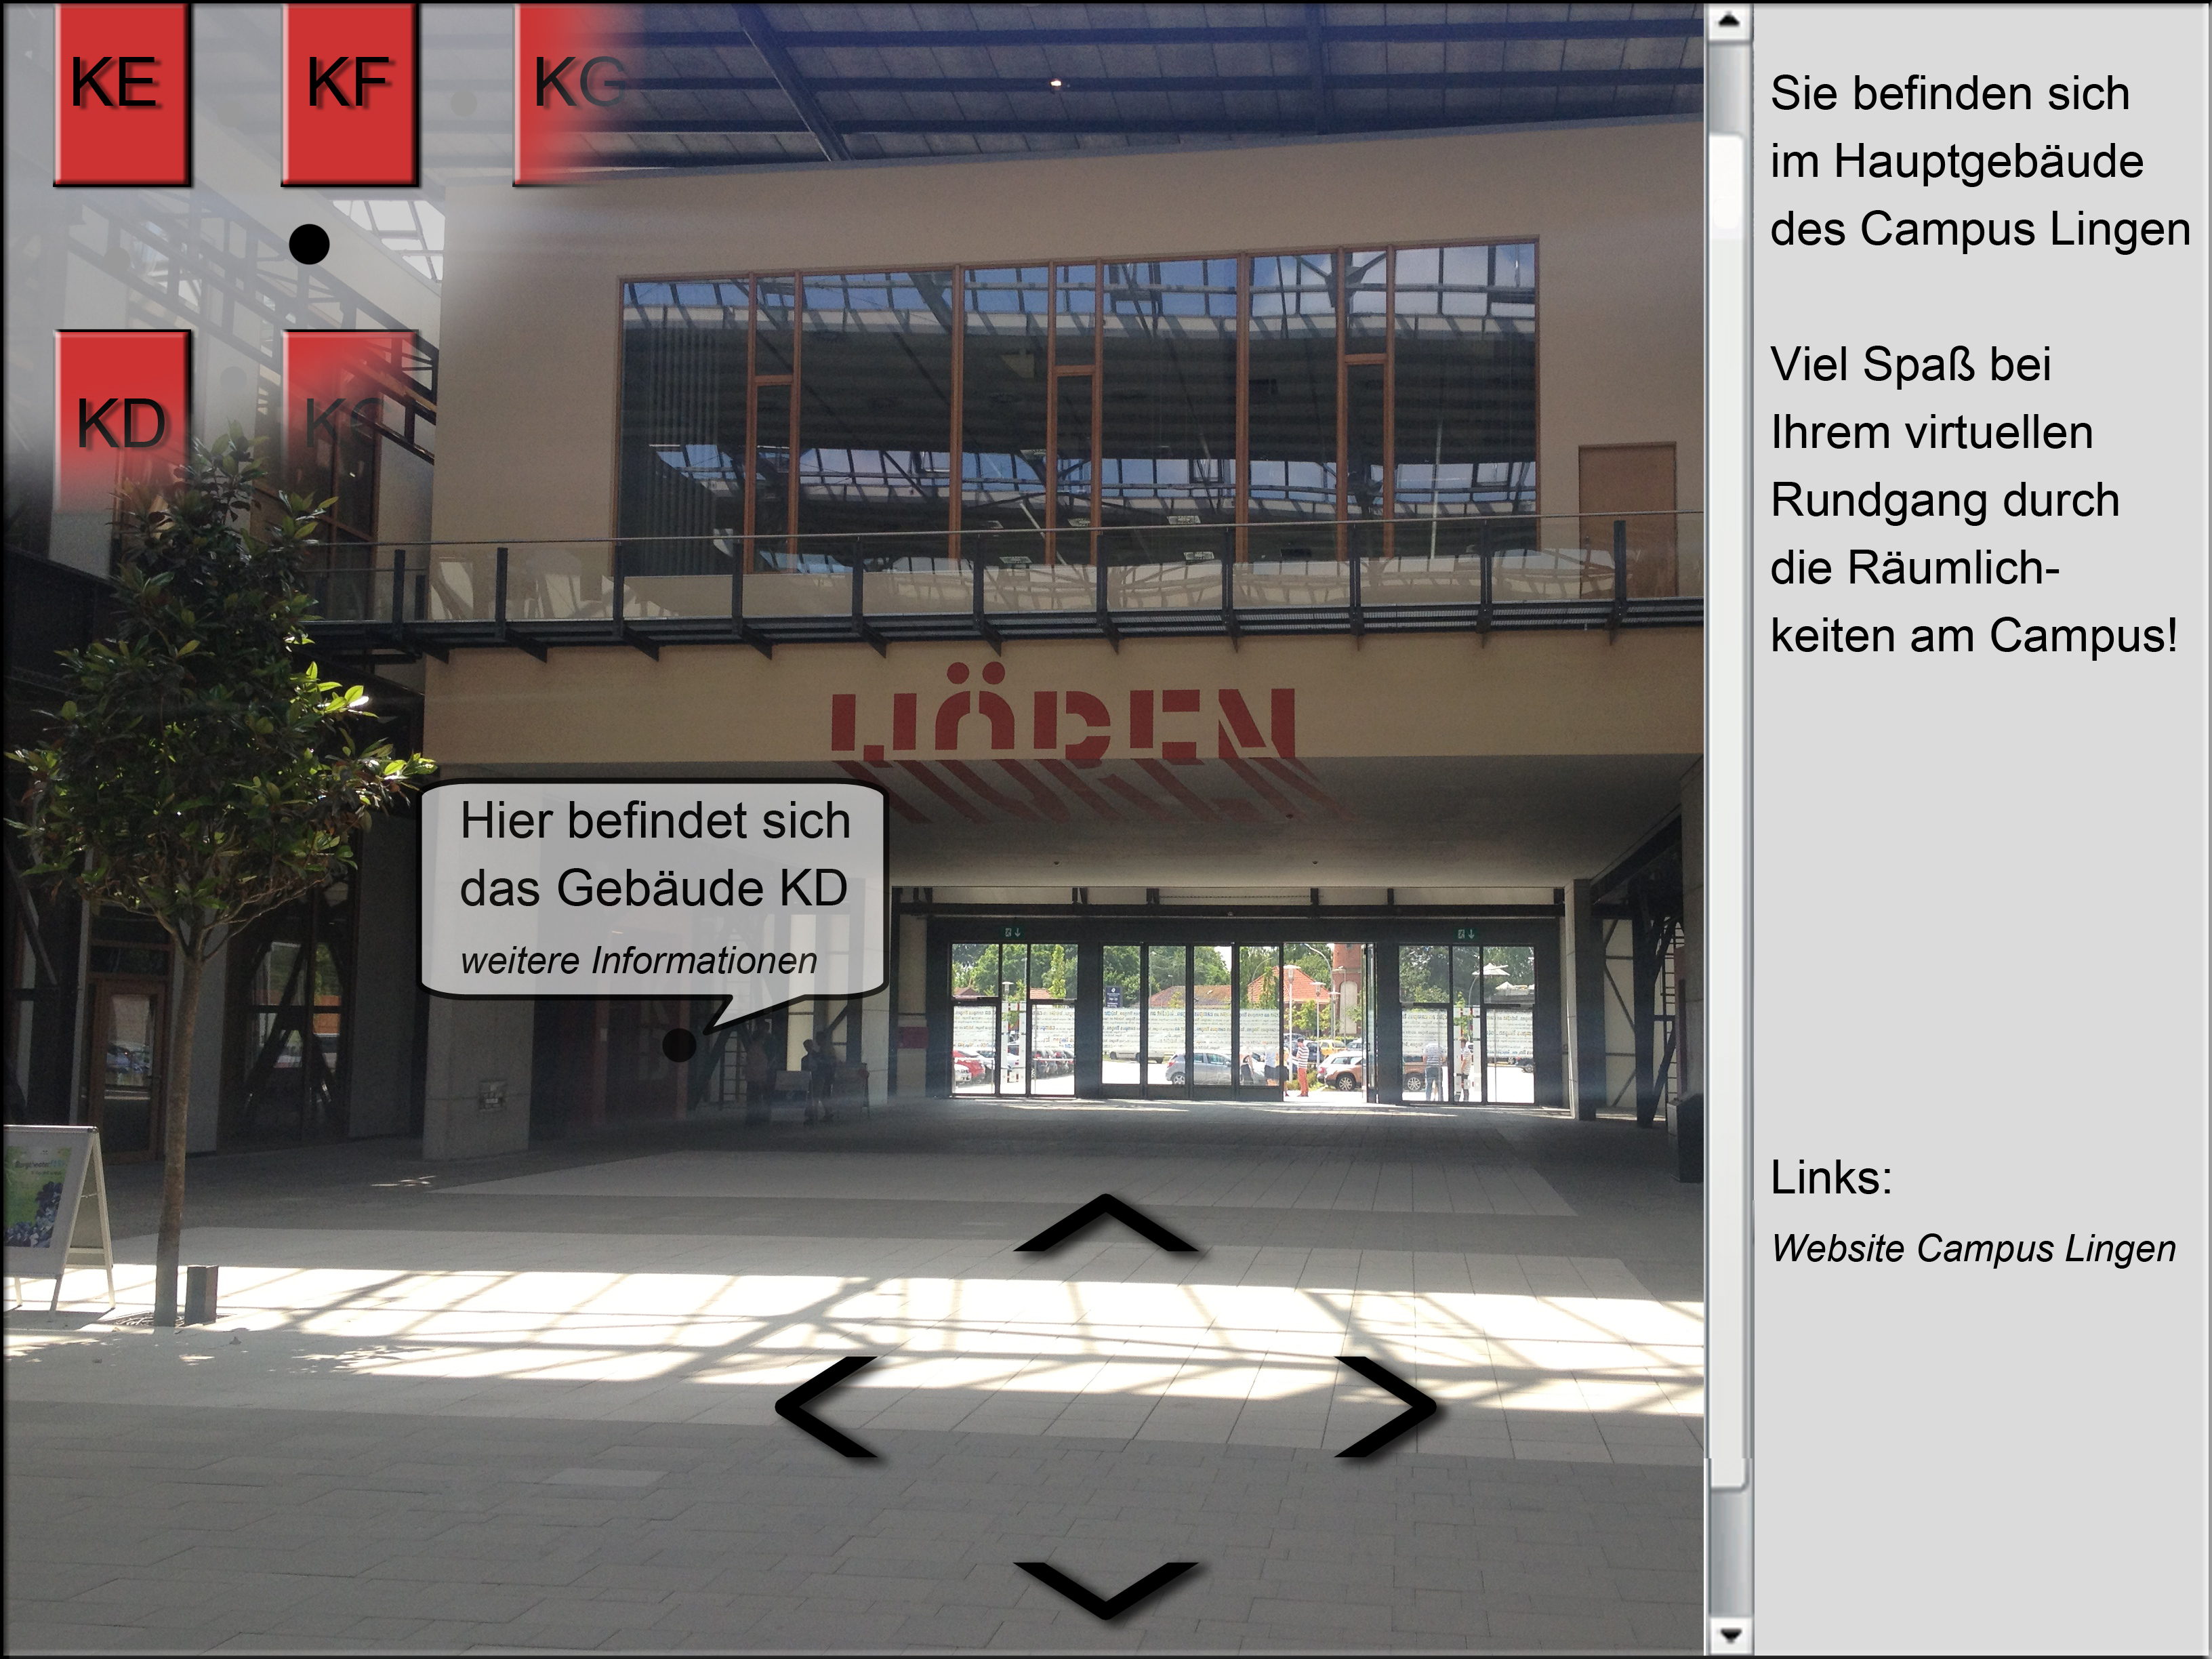
\includegraphics[width=1.0\textwidth]{MockupFrontend.jpg}
\caption[Mockup Benutzeransicht]{Oberflächenentwurf der
Benutzeransicht\protect\footnotemark}
\label{fig:MockupFrontend}
\end{figure}
\footnotetext{Quelle: Eigene Darstellung}

In diesem Mockup sind vier Elemente dargestellt, deren Funktion im Folgenden erläutert wird.

\begin{itemize}
 \item Ein 360-Grad Panorama
 \item Ein Steuerkreuz
 \item Eine kleine Übersichtskarte (Minimap)
 \item Ein Informationsfenster
\end{itemize}

Das \textbf{360-Grad Panorama} ist zentrales Element des Projektes. Dieses Panorama stellt einen Blickwinkel dar, von dem aus sich ein Benutzer den Campus Lingen ansehen kann. Von diesem Blickwinkel aus kann sich der Benutzer virtuell um die Vertikalachse der Fotoaufnahme drehen und dabei alles in diesem Blickwinkel betrachten. Er kann zudem die Aufnahme um 180-Grad horizontal drehen. Ein Benutzer hat damit von einen Standpunkt aus einen vollen Rundumblick.

Mit dem \textbf{Steuerkreuz} am unteren Rand des Panoramas kann ein Benutzer zu einem anderen Aufnahmepunkt wechseln. Er erhält damit einen Einblick aus einem anderen Blickwinkel und kann sich in diesem wiederum frei umsehen. Die Pfeile des Steuerkreuzes zeigen dabei zu jeder Panoramaaufnahme, die von der aktuellen Position erreichbar ist.

Die \textbf{Minimap} ist in einer der Ecken des Panoramas platziert und erfüllt zwei Aufgaben. Zum einen dient sie der Übersichtlichkeit und Orientierung des Benutzers. Sie zeigt an welcher Aufnahmeposition sich der Benutzer aktuell am Campus befindet (im Oberflächentwurf durch einen schwarzen Punkt gekennzeichnet). Hierdurch wird neben dem Einblick in die Räumlichkeiten des Campus auch ein Bild des Aufbaus vermittelt.
Zum anderen kann die Minimap, genau wie die Pfeile des Steuerkreuzes, zum Navigieren zu anderen Aufnahmen genutzt werden. Dazu werden alle Aufnahmepositionen, die sich im Sichtfeld des dargestellten Ausschnittes befinden, farblich hervorgehoben. Durch anklicken einer solchen Markierung wird der Benutzer in eine andere Aufnahmeposition versetzt. Beim wechseln der Aufnahmeposition verändert sich dabei auch der dargestellte Ausschnitt der Minimap.

Das \textbf{Informationsfenster} zeigt zu guter Letzt interessante Informationen zum aktuellen Panorama an. Im obigen Oberflächenentwurf sind zwei solcher Informationsfenster dargestellt (am rechten Rand und oberhalb des Steuerkreuzes). Diese Darstellungsformen sind als alternativ zu betrachten. Die Art der Informationsdarstellung ist zum Zeitpunkt des Öberflächenentwurfs noch nicht eindeutig festgelegt. Inhalt dieser Informationsfenster können dabei Interessante Projekte einzelner Studiengänge, Öffnungszeiten von Räumlichkeiten oder Wissenwertes aus dem Studienalltag sein. Die Anzeige der Informationsfenster ist dabei in einer Art Popup gedacht. Das heißt sie sollen nicht permanent angezeigt werden, sondern erscheinen erst durch Klick des Benutzers auf einen Button. Dadurch wird das Panorama und damit der Blick des Benutzers nicht durch störende Anzeigen eingeschränkt.

\clearpage